\chapter{Methodology}\label{ch:methodology}

In this chapter, the test equipment and experiment procedures are presented. The experiment is based on the planatary test rig in UNSW. Vibration signals are collected by a National Instrument data acquisition system and analysed in Matlab.

\section{Equipment}

The test equipment include the planetary gearbox test rig, control system and the data acuisition system.

\subsection{Planetary gearbox test rig}

The UNSW planetary gearbox test rig was firstly built by Sweeney in parallel configuration and then modified to planetary configuration. Seen from the layout in Figure 3.1, the test rig is driven by a 3 Phase AC induction motor and a hydraulic pump provided the resistance torque. Two flywheels are mounted on input and output shaft to minimize speed fluctuation.
Power is transfered through the planetary gearbox in the center. The planetary has a parallel stage and a planetary stage. The input of the parallel stage is a 42-tooth pinion gear, and the output is a 55-tooth spur gear fixed to the planet carrier. The planetary stage is driven by the planet carrier. It carries tree planet gears which have 23 teeth each. The ring is fixed and has 80 teeth. The output sun gear has 34 teeth.

\begin{figure}
	\centering
	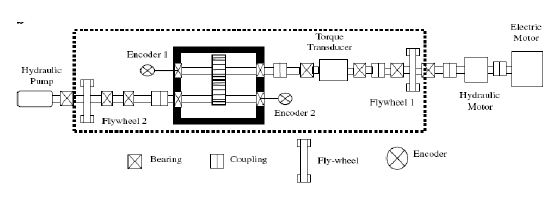
\includegraphics{rig}
	\caption{UNSW planetary gearbox test rig}
	\label{testrig}
\end{figure}

The gearbox is connected to the input and output shafts by belt couplings, which are not shown in the layout of Figure 3.1. Tension of the belts are adjusted by the sliding rails downside the gearbox housing. The planetary gearbox and the belt drives are illustrated in Figure 3.2.

A in-line torque transduser is used to measure the torque on the drive shaft. Its result is shown directly on The UNSW MK II transducer indicator. Due to the limitation of the belt transmission, the maximum torque is restricted to 70 Nm.
A Hiedhan 426-36000 shaft encoder is mounted on the input shaft of the gearbox. Which is shown on the upper-left corner of Figure 3.2. 
The external accelerometer is fixed by stud to the outframe of the ring gear. There are two internal accelerometers, axial and radial, mounted inside the spur gear. The radial transducer rotate together with the carrier, and its signal is trasferred out through a Michigan Scientific B6-2 slip ring on the left side. Both the external and internal transducers are Bruel \& Kjaer 4394 IEPE accelerometers.

\begin{figure}
	\centering
	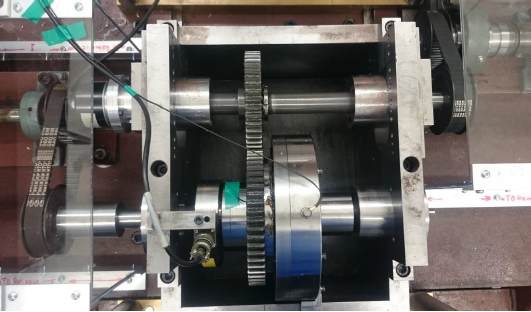
\includegraphics{gearbox}
	\caption{The planetary gearbox}
	\label{gearbox}
\end{figure}

The speed of the AC induction motor is controlled by a F		RENIC-MEGA variable frequency drive (VFD), which allow us to run the variable speed tests. As this is a 8 pole induction moter, the input frequency displayed on the variable frequency drive should be divided by four to get the drive shaft running frequency.

The VFD is installed on the control panel together with a switch and an emergency stop button. The control panel is shown in Figure 3.3. It also contains the hydraulic control valve and the hydraulic isolation valve. The risistance torque could be adjusted by the control valve.

\begin{figure}
	\centering
	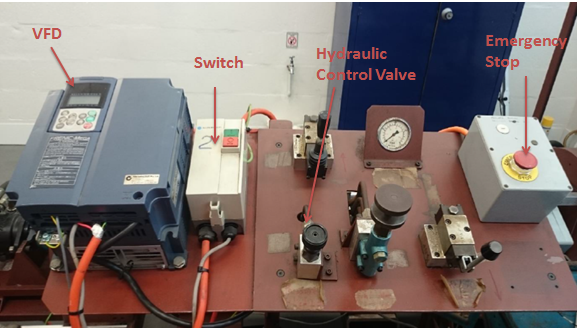
\includegraphics{control}
	\caption{The test rig control panel}
	\label{control panel}
\end{figure}

\subsection{Data acquisition system}

The test signals generated by the rig are collected by a National Instrument (NI) data acuisition system. 



\section{Test Settings}







\section{Processing and Analysis}